\documentclass[uplatex,dvipdfmx,a4paper,10pt,twocolumn]{bxjsarticle}

\usepackage[dvipdfmx]{graphicx}
\usepackage[dvipdfmx,colorlinks=true,allcolors=blue!55!black]{hyperref}
\usepackage{amsmath,amssymb,bm,booktabs,array,multirow}
\usepackage{geometry}
\usepackage{xcolor}
\usepackage{url}
\usepackage{enumitem}

\geometry{top=18mm,bottom=20mm,left=17mm,right=17mm}
\setlength{\columnsep}{6mm}
\setlength{\textfloatsep}{8pt plus 2pt minus 2pt}
\setlength{\floatsep}{7pt plus 2pt minus 2pt}
\setlength{\intextsep}{7pt plus 2pt minus 2pt}
\setlist[itemize]{leftmargin=1.5em,itemsep=1pt,topsep=2pt}
\graphicspath{{figures/}}

\newcommand{\R}{\mathbb{R}}
\newcommand{\RSN}{RSN}
\newcommand{\knn}{KNN}
\newcommand{\good}{\mathop{\uparrow}}
\newcommand{\low}{\mathop{\downarrow}}

\title{\RSN：クラス条件付きロバスト標準化近傍距離による\\
野生動物画像の超近接分布外検知}
\author{表 紘太朗\\
慶應義塾大学 総合政策学部\\
\texttt{kotaro3150@keio.jp}}
\date{}

\begin{document}
\maketitle

\begin{abstract}
既知クラスと未知クラスが同一の細粒度カテゴリに属する場合，未知入力は凍結特徴空間で既知クラスの近傍に入り込み，通常の分布外（out-of-distribution; OOD）検知は難しくなる．本稿では，この超近接 OOD 設定に対し，\RSN（Robust Scale-Normalized kNN）を提案する．\RSN は，生の DINOv2 特徴をクラスごとの次元別標準偏差で正規化し，クラス別に取得した $k=150$ 近傍との残差を Huber 関数で集約する．主設定は特徴の $\ell_2$ 正規化，分類 head による候補クラス制限，経験分位点較正をいずれも用いない．重複・明白な誤画像を除いたネコ科8種・105,554枚のデータセットで，ID クラス数 $m=2,\ldots,7$ の全組合せ，3 seed，2 backbone を評価した．$m=2$ の検証済み再実験では，\RSN は AUROC 0.9169，FPR95 0.4307，AUPR-OUT 0.9590を達成し，\knn の0.9126，0.4626，0.9560を上回った．また全 $m$ で \knn および PSM より高い AUROC と低い FPR95を示した．さらに，ベースライン実装を原論文の定義と照合し，raw score fingerprint と fold 完備性を監査した結果のみを報告する．
\end{abstract}

\section{はじめに}

深層画像分類器は，学習時に観測していない入力に対しても高い確信度を返すことがある~\cite{hendrycks2017baseline}．この問題を扱う OOD 検知は，分類結果を生態調査や保全判断へ接続する野生動物認識で特に重要である~\cite{norouzzadeh2018automatically,tuia2022perspectives}．誤った既知種判定は，個体数推定，希少種発見，外来種監視の下流処理へそのまま伝播するためである．

従来の評価では，ID と OOD が視覚的に大きく異なる設定も多い．一方，実際の種同定では，未知種が既知種と同じ科に属し，体型，毛皮模様，姿勢，背景が強く類似する．本研究では，このように同一ドメイン・同一分類群の種のみで ID/OOD を構成する設定を\textbf{超近接 OOD（Ultra-Near-OOD）}と呼ぶ．対象は cheetah，jaguar，leopard，lion，ocelot，puma，serval，tiger の8種であり，jaguar，leopard，ocelot のロゼット模様など，未知種を既知種へ近づける視覚要因を含む．

凍結特徴に対する \knn は，分類 head に依存せず，局所密度を利用できる強い基準である~\cite{sun2022knn}．しかし通常の \knn は，すべてのクラスを同一の等方的距離で測る．姿勢や背景の変動が大きいクラスと均質なクラスでは，各特徴次元の自然な変動幅が異なるため，生の距離はクラス間で同じ意味を持たない．また低分散な一方向だけの偶発的なずれが，標準化距離全体を過度に押し上げる場合がある．

そこで本稿では \RSN を提案する．本研究の貢献は次の3点である．
\begin{itemize}
  \item クラス条件付き次元別標準化と Huber 集約を組み合わせた，学習不要・較正不要の近傍 OOD score を定義する．
  \item 105,554枚のクリーニング後データで，全 ID 組合せ $\times$ 3 seed $\times$ 2 DINOv2 backbone，計1,476 foldを評価し，$m=2$ から7まで一貫した \knn/PSM 超えを示す．
  \item 比較実装を再監査し，誤 dispatch，別名重複，cached DINOv2 特徴だけでは原定義を再現できない手法を除外した検証済み表を提示する．
\end{itemize}

\section{関連研究}

\subsection{分類 head に基づく OOD 検知}

MSP~\cite{hendrycks2017baseline} は最大 softmax 確率を ID らしさとする．Energy~\cite{liu2020energy}，MaxLogit，Entropy，GEN~\cite{liu2023gen} は，同じ logit から異なる集約を構成する．GradNorm~\cite{huang2021gradnorm} は分類層勾配，OpenMax~\cite{bendale2016openmax} は EVT による未知クラス確率を用いる．これらは軽量である一方，ID クラス間識別のための head が超近接 OOD に高い logit を与えると，score 全体が影響を受ける．本稿では共通の決定論的 ridge 線形 head を用い，head 依存手法間の学習条件を揃える．

\subsection{特徴距離に基づく OOD 検知}

Mahalanobis 法~\cite{lee2018simple} はクラス条件付きガウス分布を仮定し，共有共分散による距離を用いる．RMD~\cite{ren2021simple} はクラス距離から背景分布の距離を差し引き，Mahalanobis++~\cite{muller2025mahalanobispp} は特徴正規化を導入する．ViM~\cite{wang2022vim} は分類 logit と特徴残差を結合する．\knn~\cite{sun2022knn} は分布形の仮定を置かず，正規化特徴の近傍距離を用いる．

\RSN は \knn と同じ近傍探索を基礎とするが，距離をクラスごとの次元別スケールへ適応させる．フル共分散の逆行列を推定せず，$D$ 個の標準偏差だけを推定する点で Mahalanobis 系とも異なる．さらに，標準化後の各座標を二乗和へ直接入れず Huber 化し，単一座標の影響を抑える．

\section{提案手法}

図~\ref{fig:pipeline} に主設定の処理を示す．重要なのは，旧実験で実際に用いられ，検証済み再実験でも最良だった設定を主役とする点である．すなわち，\textbf{生の DINOv2 特徴，$k=150$，全 ID クラス候補，Huber $\delta=1.345$，較正なし}を用いる．

\begin{figure*}[t]
  \centering
  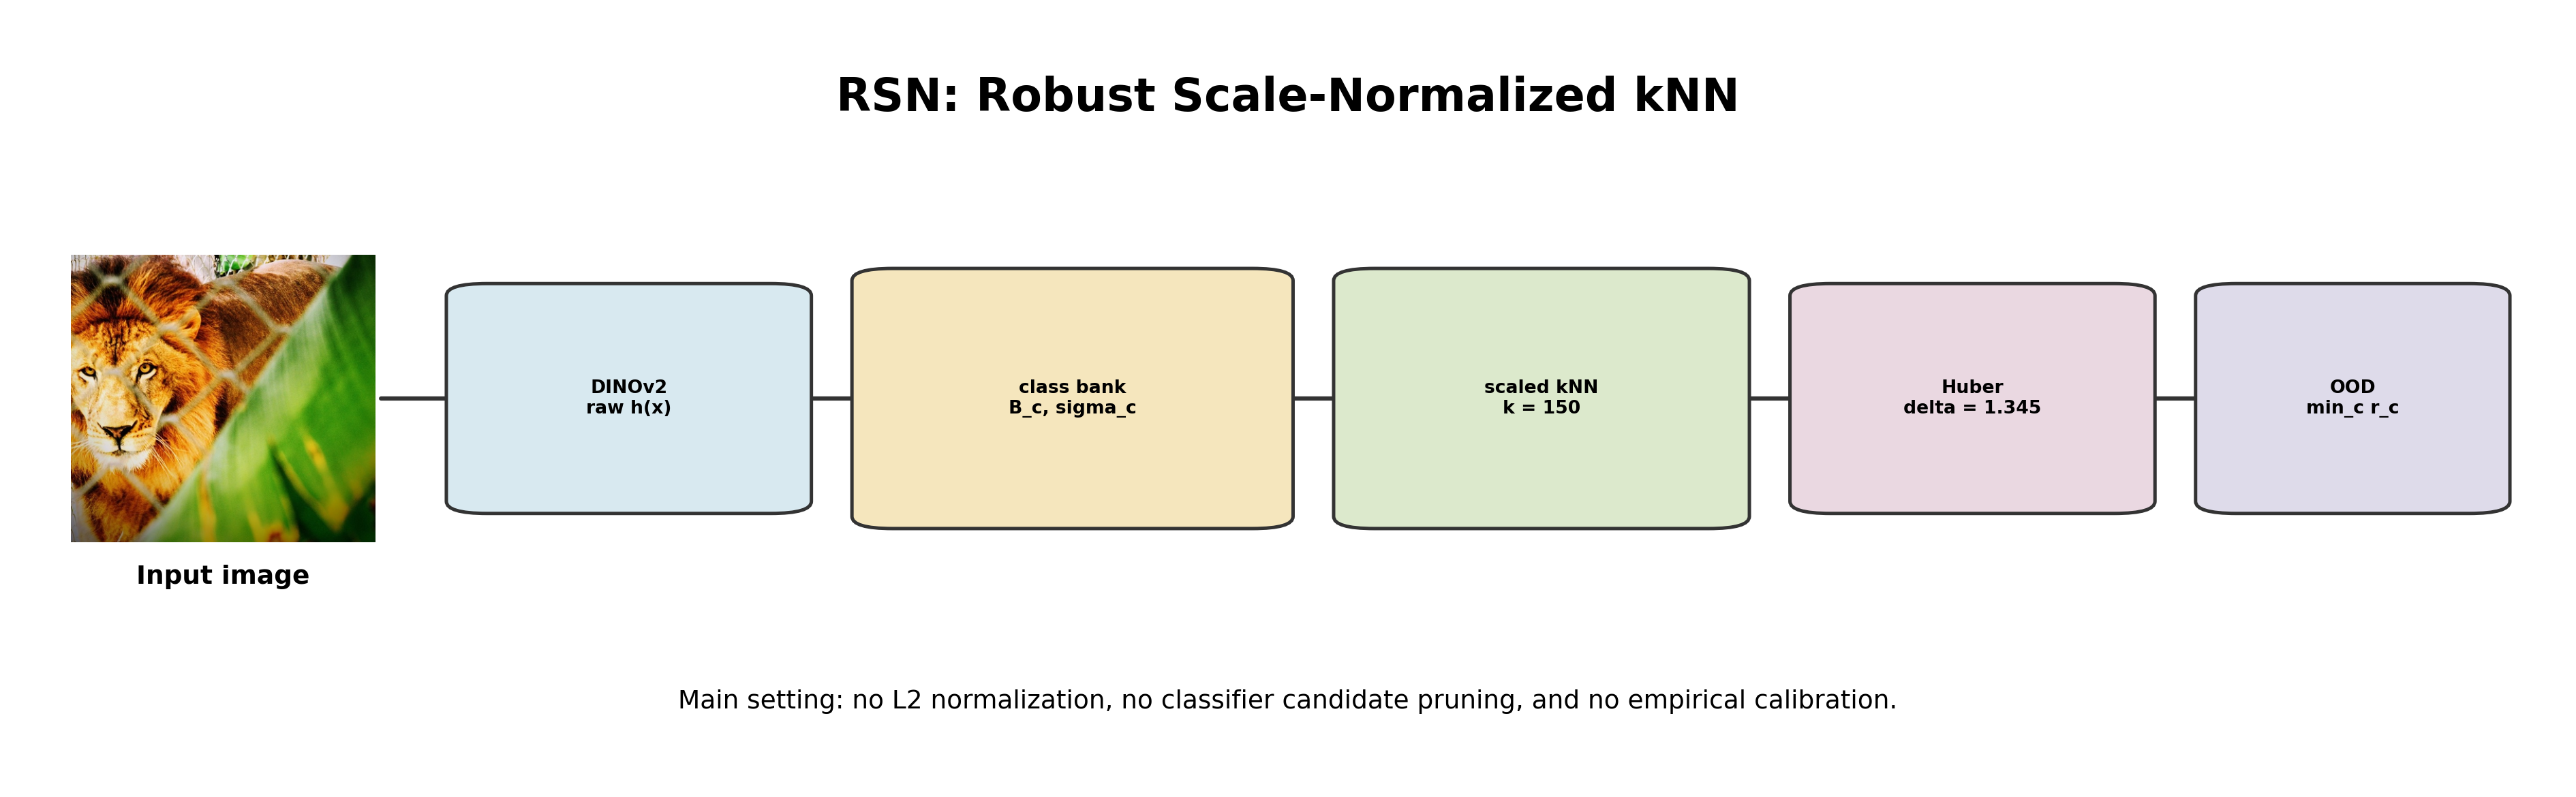
\includegraphics[width=0.98\textwidth]{fig01_rsn_old_pipeline.png}
  \caption{\RSN の主設定．生の DINOv2 CLS 特徴からクラス別バンクと次元別標準偏差を作り，各クラスで標準化後の150近傍を求める．Huber 集約後，すべての ID クラスに対する最小距離を OOD score とする．$\ell_2$ 正規化，top-$q$ 候補制限，経験分位点較正は用いない．}
  \label{fig:pipeline}
\end{figure*}

\subsection{生特徴とクラス別スケール}

凍結 backbone の CLS 特徴を
\begin{equation}
  h(x)\in\R^D
\end{equation}
とし，主設定では $\ell_2$ 正規化しない．ID クラス $c$ の train 特徴バンクを
\begin{equation}
  \mathcal{B}_c=\{h_i\mid y_i=c\}
\end{equation}
とする．各次元 $d$ の標準偏差は
\begin{equation}
  \sigma_{c,d}=\max\!\left(\mathrm{std}\{h_i^{(d)}:h_i\in\mathcal{B}_c\},\tau\right),
  \quad \tau=10^{-3}
  \label{eq:sigma}
\end{equation}
で推定する．対角スケールだけを用いるため，推定パラメータ数はクラスあたり $D$ であり，共分散の $O(D^2)$ パラメータや逆行列を必要としない．

\subsection{標準化近傍と Huber 集約}

クラス $c$ に対し，問い合わせとバンクをそれぞれ $\bm{h}/\bm{\sigma}_c$ で標準化し，Euclidean 距離が小さい $k=150$ 点の添字集合を $N_k^c(x)$ とする．近傍 $i$ の次元別残差は
\begin{equation}
  t_{c,i}^{(d)}(x)=\frac{h^{(d)}(x)-h_i^{(d)}}{\sigma_{c,d}}.
\end{equation}
標準化により低分散次元のずれを検出しやすくなる一方，単一次元の偶発的な外れ値も増幅される．そこで実装と一致する Huber 型関数
\begin{equation}
\rho_\delta(t)=
\begin{cases}
t^2,& |t|\le\delta,\\
2\delta|t|-\delta^2,& |t|>\delta
\end{cases},\qquad \delta=1.345
\label{eq:huber}
\end{equation}
を用いる~\cite{huber1964robust}．クラス距離は
\begin{equation}
  r_c(x)=\frac{1}{k}\sum_{i\in N_k^c(x)}\sum_{d=1}^{D}
  \rho_\delta\!\left(t_{c,i}^{(d)}(x)\right)
  \label{eq:classdistance}
\end{equation}
である．$\rho$ は小さい残差を二乗で保持し，大きい残差を線形へ切り替える．

\subsection{OOD score}

最終 score は全 ID クラスに対する最小値
\begin{equation}
  o_{\RSN}(x)=\min_{c\in\mathcal{C}_{\mathrm{ID}}}r_c(x)
  \label{eq:score}
\end{equation}
とし，大きいほど OOD とする．分類 head の top-$q$ で候補を削らないため，head の誤分類で正しい近傍クラスが除外されない．全バンクを走査する主項は通常の brute-force \knn と同じ $O(ND)$ で，その後の Huber 集約は $O(CkD)$ である．実験では GPU 上でクラス・問い合わせを batch 化する．

\subsection{較正を用いない理由}

クラス特徴が $h_c=\mu_c+\sigma_c\odot u$，かつ潜在分布 $u$ がクラス間で共有されるなら，式~\eqref{eq:sigma}の標準化後は $r_c$ の ID 分布が共通分布 $F$ に近づく．このとき経験分位点 $q_c(x)=1-F(r_c(x))$ を追加しても，
\begin{equation}
  \arg\max_c q_c(x)=\arg\min_c r_c(x)
\end{equation}
であり，score の単調変換にすぎない．有限 validation からクラス別 $\hat F_c$ を再推定すると，DKW 不等式~\cite{dkw1956}
\begin{equation}
  \Pr\!\left(\sup_r|\hat F_c(r)-F_c(r)|>\epsilon\right)
  \le 2e^{-2n_c\epsilon^2}
\end{equation}
の推定誤差がクラスごとに加わる．したがって，対角標準化でスケール差が十分小さくなった場合，較正は情報利得より順位ノイズを増やしうる．実験ではこの仮説を4条件 ablation と分布形状の直接比較で検証する．

\section{実験設定}

\subsection{CAT データセット}

ウェブ収集画像に対し，完全重複・近重複のグループ化と，明白な別内容，足跡のみ，地図・画面等の除外を行った．最終枚数は表~\ref{tab:counts}の105,554枚である．自動クリーニング後も誤ラベルが完全にゼロとは仮定しないが，実験に用いた manifest の実測枚数は期待値と全クラスで一致した．重複群が train/validation/test を跨がないよう，クラス内で4:1:1に分割した．

\begin{table}[t]
\centering
\caption{クリーニング後 CAT データセット．}
\label{tab:counts}
\begin{tabular}{lr@{\hspace{7mm}}lr}
\toprule
種 & 枚数 & 種 & 枚数\\
\midrule
cheetah & 11,349 & ocelot & 12,342\\
jaguar  & 10,452 & puma   & 18,763\\
leopard & 10,984 & serval &  9,149\\
lion    & 15,845 & tiger  & 16,670\\
\midrule
\multicolumn{3}{r}{合計} & 105,554\\
\bottomrule
\end{tabular}
\end{table}

8種から $m=2,3,4,5,6,7$ 種を ID として選び，残りを OOD とする全組合せを評価した．seed は0,1,2，backbone は DINOv2 ViT-B/14 と ViT-L/14~\cite{oquab2024dinov2}である．fold 数は各 $m$ で168，336，420，336，168，48，合計1,476となる．OOD train/validation は用いず，protocol は fair のみとした．

\subsection{比較手法と実装監査}

主比較は \knn（正規化特徴，$k=50$）と PSM（$r=48,k=200$）である．$m=2$ では，MSP，Entropy，Energy，MaxLogit，GEN，GradNorm，KL-Matching，Mahalanobis，Mahalanobis++，RMD，ViM，ReAct，ASH-P/B/S，DICE，SCALE，NCI，OpenMax も同一 fold で再実行した．分類器依存手法はすべて，ID train の生 DINOv2 特徴に閉形式 ridge 線形 probe（$\lambda=10^{-3}$，bias は非正則化）を学習して使用した．early stopping は行わない．

比較の信頼性を確保するため，原論文の score 定義，dispatch，特徴正規化，共分散，分類 head を再点検した．ODIN は入力勾配と摂動を cached 特徴から再現できず，CLIP zero-shot/MCM/Tip-Adapter は CLIP image-text encoder を用いない限り原手法ではないため，DINOv2 表から除外した．`mah\_mindist' は nearest-class Mahalanobis の別名であり独立行としない．全 fold で method 別 raw score の SHA-256 fingerprint を保存し，欠測・重複・非有限値を検査した．

\subsection{評価指標}

OOD を positive とし，AUROC$\good$，FPR95$\low$，AUPR-OUT$\good$ を報告する．表の平均は fold-level 指標の算術平均である．手法比較では backbone，seed，ID set を揃えた paired 差を用い，$t$ 分布近似の95\%信頼区間と good rate（\RSN が改善した fold 比率）を求めた．

\section{結果}

\subsection{検証済み $m=2$ 比較}

表~\ref{tab:verifiedtop} と図~\ref{fig:ranking}に，実装監査後の $m=2$ 結果を示す．\RSN は3指標すべてで最良であり，\knn に対して AUROC $+0.00426$，FPR95 $-0.03192$，AUPR-OUT $+0.00302$ である．特徴距離系では ViM，Mahalanobis，Mahalanobis++ が続く．

\begin{table}[t]
\centering
\footnotesize
\caption{検証済み上位手法（$m=2$, pooled, $n=168$）．}
\label{tab:verifiedtop}
\begin{tabular}{clrrr}
\toprule
順位 & 手法 & AUROC & FPR95 & AUPR\\
\midrule
1 & \textbf{\RSN} & \textbf{.9169} & \textbf{.4307} & \textbf{.9590}\\
2 & \knn & .9126 & .4626 & .9560\\
3 & ViM & .9041 & .5436 & .9482\\
4 & Mahalanobis & .9010 & .5474 & .9470\\
5 & Mahalanobis++ & .8987 & .5618 & .9453\\
6 & DICE & .8792 & .7230 & .9292\\
\bottomrule
\end{tabular}
\end{table}

\begin{figure*}[t]
  \centering
  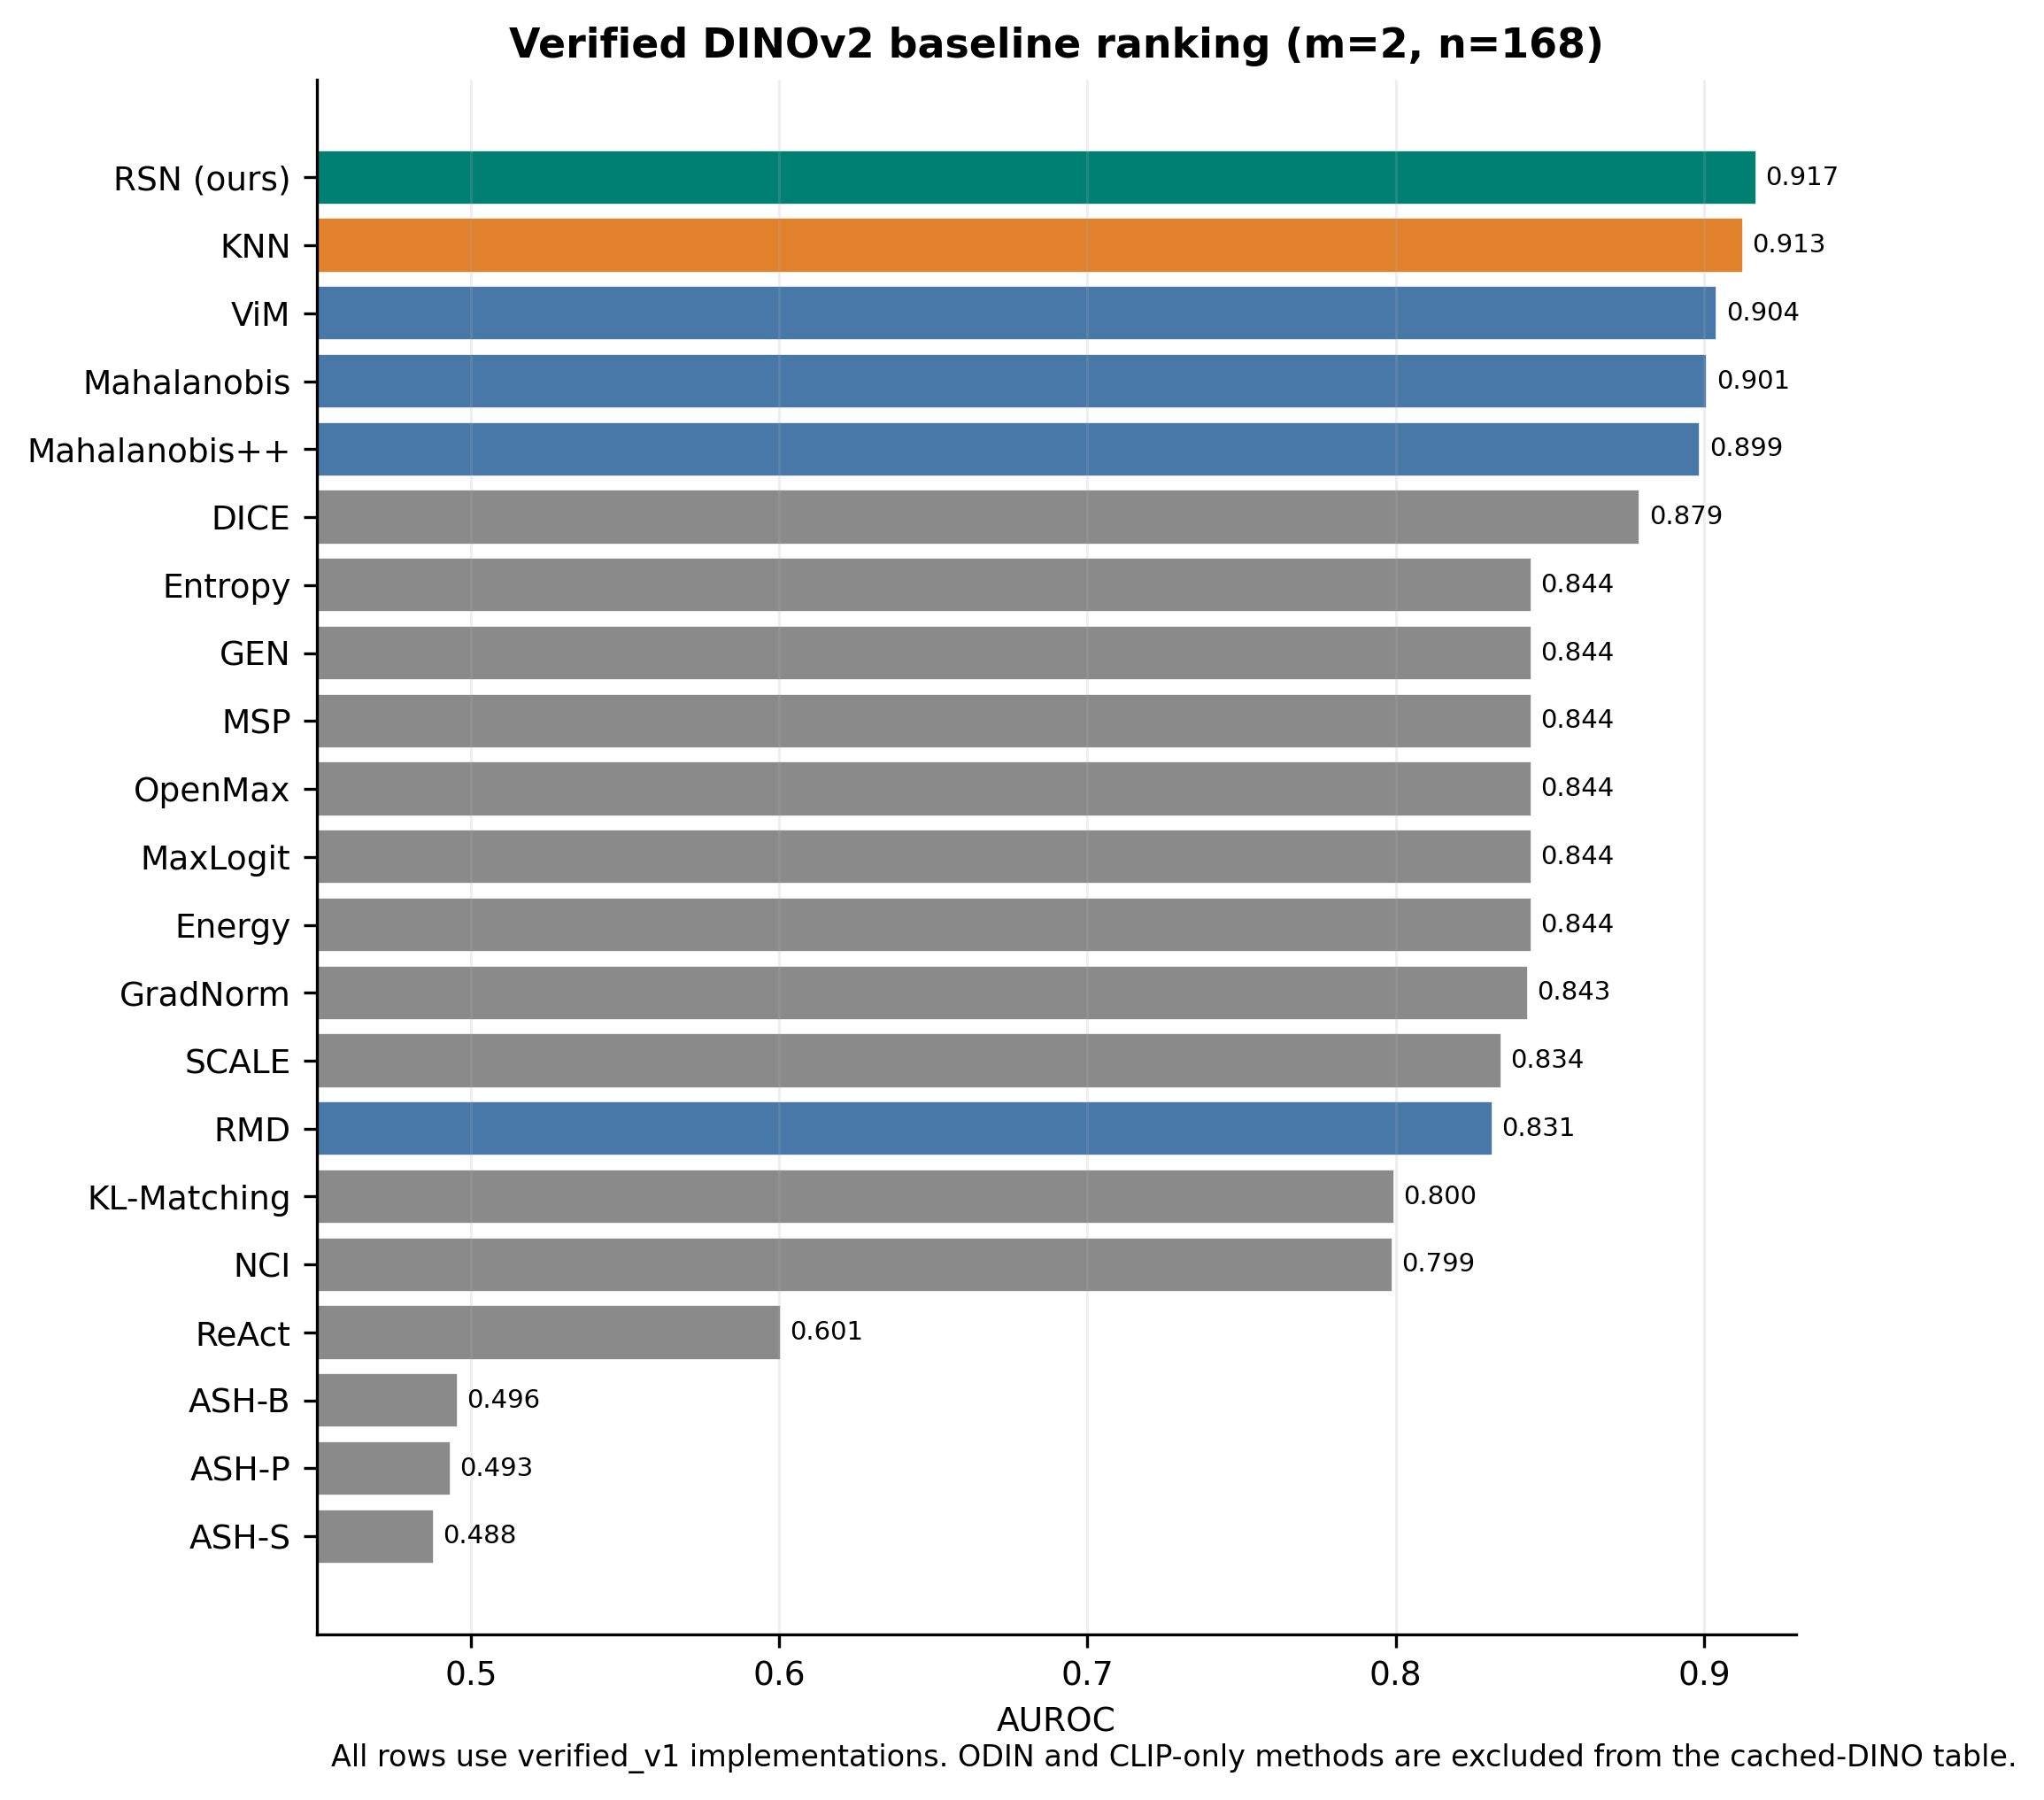
\includegraphics[width=0.78\textwidth]{fig03_verified_ranking.png}
  \caption{$m=2$ の検証済み DINOv2 手法 AUROC．\RSN の別設定は感度分析に回し，主ランキングには1行だけ掲載した．全数値は `verified\_v1' 実装による．}
  \label{fig:ranking}
\end{figure*}

MSP，Entropy，GEN は平均3指標が同じ値（AUROC 0.8440）になったが，raw score fingerprint は全168 foldで異なる．ID が2クラスの場合，これらは同じ絶対 logit margin の単調関数になり，二値 OOD ranking が一致しうるためである．したがって，この一致は dispatch 重複ではない．一方，監査前に見られた Mahalanobis 系の完全一致は修正後に解消した．

\subsection{ID クラス数と backbone}

表~\ref{tab:idsize}および図~\ref{fig:idsize}に全 $m$ の結果を示す．\RSN は $m=2$ から7まで，\knn と PSM の両方に対して AUROC が高く，FPR95 が低い．ID クラスが増えるほど OOD 側の残りクラスが減り，難しいロゼット種が評価に占める組合せ効果も強くなるため，全手法の絶対性能は低下する．ただし相対順位は維持される．

\begin{table*}[t]
\centering
\scriptsize
\caption{ID クラス数別の主比較（2 backbone pooled）．A=AUROC，F=FPR95．}
\label{tab:idsize}
\begin{tabular}{crrrrrrr}
\toprule
$m$ & $n$ & \multicolumn{2}{c}{\RSN} & \multicolumn{2}{c}{\knn} & \multicolumn{2}{c}{PSM}\\
 & & A & F & A & F & A & F\\
\midrule
2 & 168 & .9169 & .4307 & .9126 & .4626 & .9014 & .5403\\
3 & 336 & .8965 & .5005 & .8910 & .5373 & .8718 & .6468\\
4 & 420 & .8788 & .5528 & .8729 & .5951 & .8472 & .7189\\
5 & 336 & .8624 & .5952 & .8565 & .6401 & .8255 & .7677\\
6 & 168 & .8454 & .6336 & .8397 & .6835 & .8044 & .8062\\
7 &  48 & .8224 & .6857 & .8171 & .7355 & .7774 & .8445\\
\bottomrule
\end{tabular}
\end{table*}

\begin{figure*}[t]
  \centering
  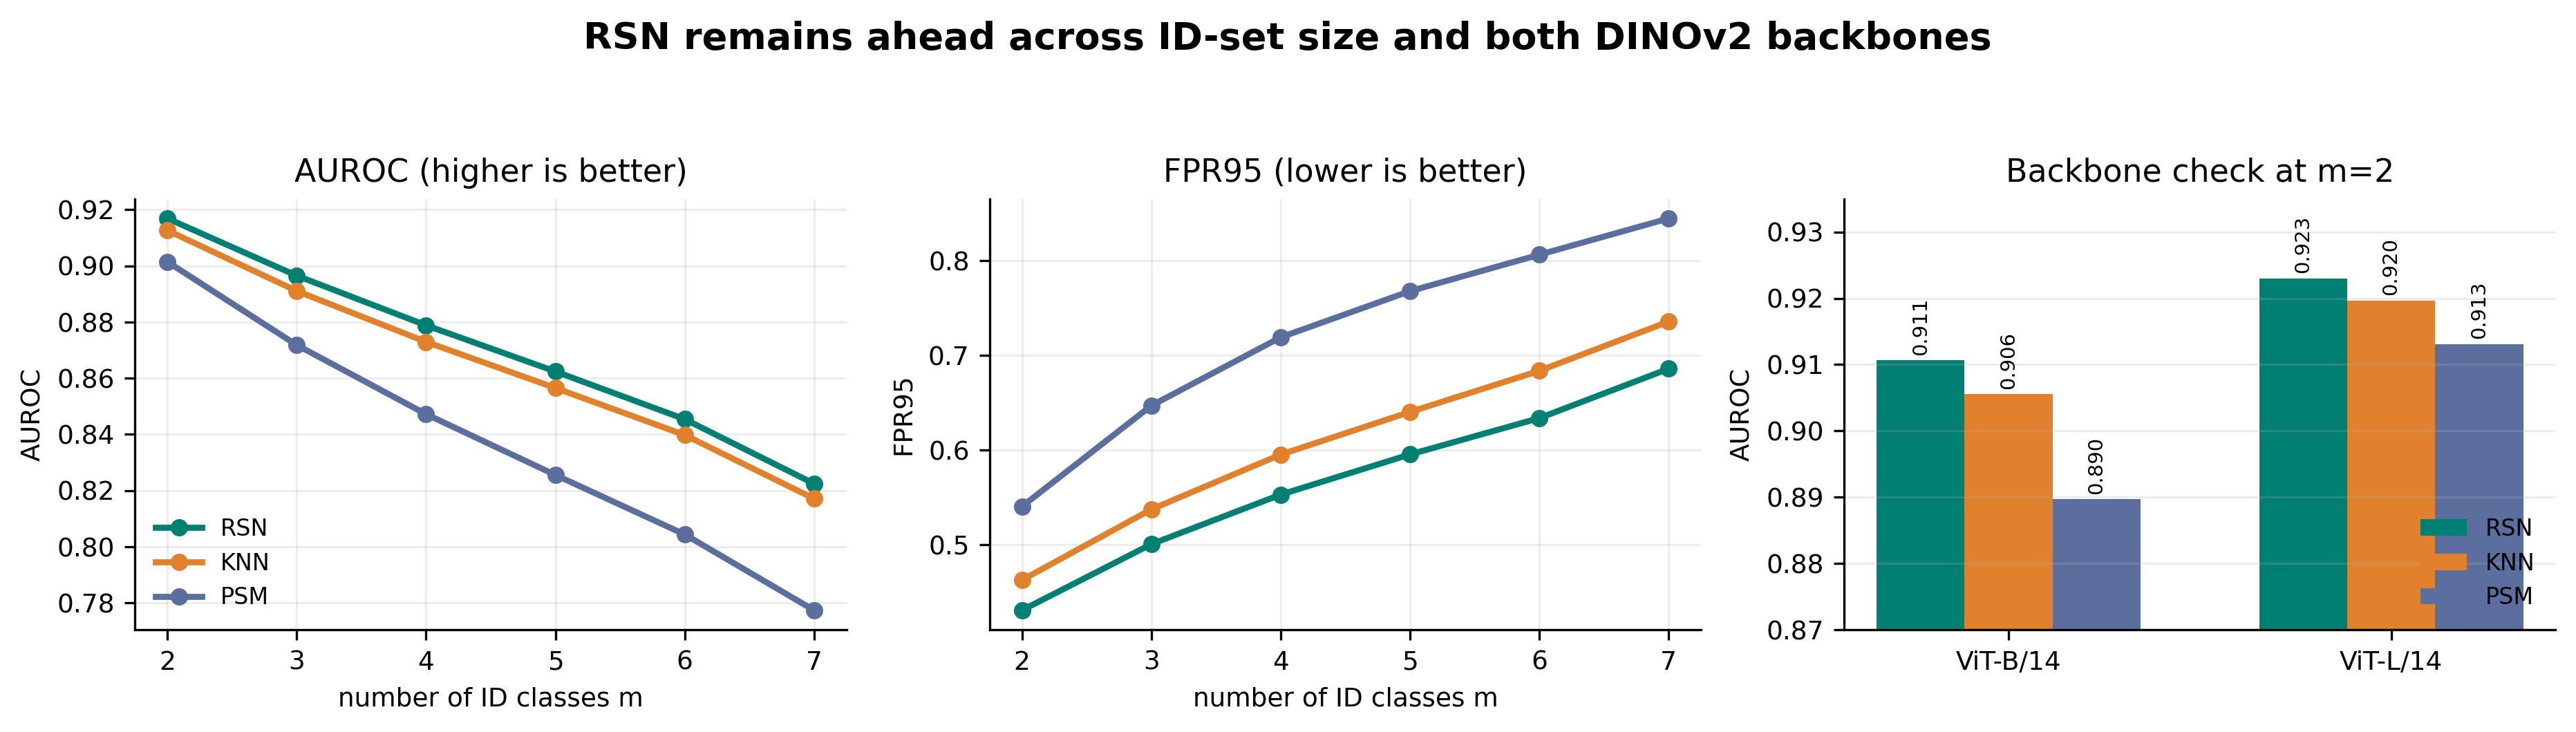
\includegraphics[width=0.98\textwidth]{fig02_idsize_backbone.png}
  \caption{左・中央：ID クラス数 $m$ に対する pooled AUROC/FPR95．右：$m=2$ の backbone 別 AUROC．\RSN は全 $m$ と両 backbone で比較手法を上回る．}
  \label{fig:idsize}
\end{figure*}

$m=2$ の ViT-B/14 では \RSN/\knn/PSM の AUROC は0.9107/0.9055/0.8897，ViT-L/14では0.9230/0.9197/0.9131であり，モデル規模によらず順位が一致した．全 $m$ の backbone 別でも同じ順位である．

\subsection{主設定の選択と ablation}

表~\ref{tab:ablation}に較正と Huber の2$\times$2 ablation，および旧PDFで一時的に記述されていた $\ell_2$ 正規化・$k=10$・top-3設定を示す．最良は旧実験の実設定，すなわち本稿の \RSN である．$\ell_2$/10/top-3設定は AUROC 0.9086で \knn を下回るため，主設定として扱わない．この差は，特徴ノルム情報の除去，局所近傍数の減少，head による候補誤除外を同時に含む設定感度であり，単一要因の効果とは解釈しない．

\begin{table}[t]
\centering
\scriptsize
\caption{設定・較正・Huber ablation（$m=2$, $n=168$）．}
\label{tab:ablation}
\begin{tabular}{lrrr}
\toprule
設定 & AUROC & FPR95 & AUPR\\
\midrule
\textbf{\RSN (raw, $k=150$, all)} & \textbf{.9169} & \textbf{.4307} & \textbf{.9590}\\
\RSN$-$Huber & .9164 & .4362 & .9583\\
\RSN$+$calib$+$Huber & .9126 & .4706 & .9563\\
\RSN$+$calib & .9119 & .4776 & .9555\\
$\ell_2$, $k=10$, top-3 & .9086 & .4522 & .9561\\
\knn & .9126 & .4626 & .9560\\
\bottomrule
\end{tabular}
\end{table}

全1,476 foldで \RSN と \RSN$-$Huber を paired 比較すると，AUROC $+0.000363$（95\% CI $[0.000344,0.000382]$），FPR95改善 $0.005766$（$[0.005448,0.006085]$），AUPR $+0.001773$（$[0.001702,0.001844]$）であった．効果量は小さいが方向は安定し，good rate はそれぞれ87.7\%，88.1\%，97.7\%である．

\subsection{全fold paired 比較}

表~\ref{tab:paired}は全 $m$ を併合した paired 結果である．FPR95については「比較手法の FPR95 $-$ \RSN の FPR95」を改善量として正値で表す．\RSN は \knn に対して平均 AUROC $+0.00556$，FPR95を0.04156改善し，PSMに対する差はさらに大きい．

\begin{table}[t]
\centering
\scriptsize
\caption{全fold paired 比較（$n=1,476$）．}
\label{tab:paired}
\begin{tabular}{llrrr}
\toprule
比較 & 指標 & 平均改善 & 95\% CI & good\\
\midrule
\multirow{3}{*}{vs. \knn}
 & AUROC & .00556 & [.00494,.00618] & 70.0\%\\
 & FPR95 & .04156 & [.03817,.04495] & 72.2\%\\
 & AUPR & .01163 & [.01056,.01270] & 71.5\%\\
\midrule
\multirow{3}{*}{vs. PSM}
 & AUROC & .03091 & [.02958,.03223] & 91.6\%\\
 & FPR95 & .15711 & [.15126,.16297] & 95.7\%\\
 & AUPR & .05439 & [.05198,.05680] & 97.2\%\\
\bottomrule
\end{tabular}
\end{table}

18比較（6 id size $\times$ 3比較対象）を想定した Bonferroni 水準 $\alpha/18$ でも，$m=2$--6の \RSN vs. \knn は3指標で有意であった．$m=7$ は $n=48$ と小さく，\knn 比の区間が0を跨ぐため，このサイズ単独の有意性は主張しない．

\subsection{未知種別の難しさ}

図~\ref{fig:perood}に $m=2$ の per-OOD-class 結果を示す．tiger と lion は比較的分離しやすい一方，jaguar，leopard，ocelot は AUROC 0.840--0.847に留まる．3種はいずれもロゼット模様を持ち，既知側に別の斑紋種が含まれる fold で視覚的近傍へ入りやすい．ocelot の FPR95 0.711は特に高く，平均 AUROCだけでは見えない閾値近傍の誤受理が残る．

\begin{figure*}[t]
  \centering
  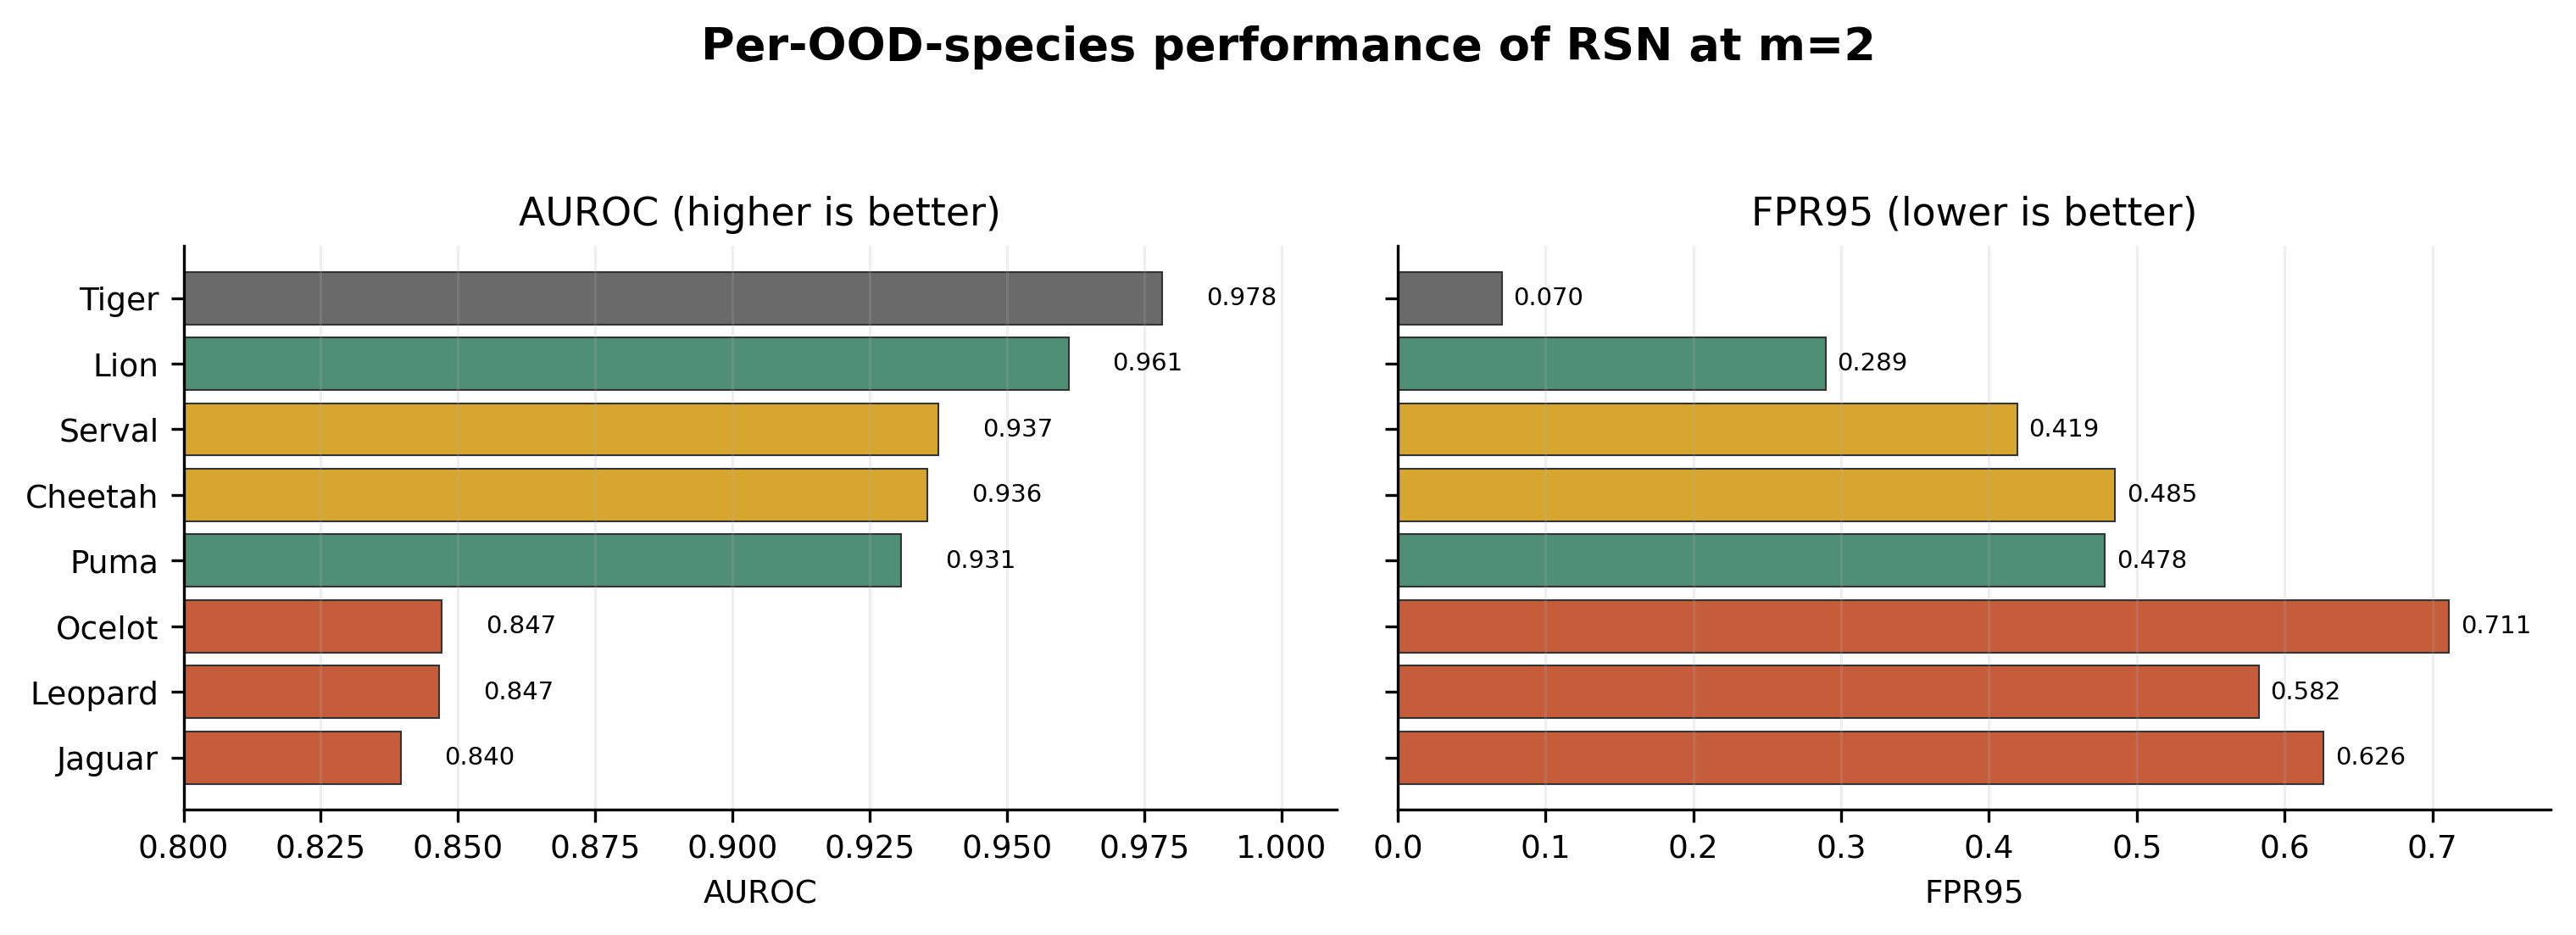
\includegraphics[width=0.90\textwidth]{fig04_per_ood_m2.png}
  \caption{$m=2$ における \RSN の未知種別 AUROC/FPR95．橙はロゼット，黄は斑点，緑は無地，灰は縞を表す．}
  \label{fig:perood}
\end{figure*}

\section{分析と考察}

\subsection{対角標準化と較正冗長性}

共有形状仮定を直接確認するため，各 fold の ID validation に式~\eqref{eq:classdistance}を適用し，クラス対の経験 CDF 間 KS 統計量と，クラス平均距離の変動係数（CV）を求めた．全fold平均は KS 0.1344，CV 0.0464であった．図~\ref{fig:cdf}の代表 foldでも CDF の中心は概ね重なり，対角標準化後のクラス平均スケール差が約4.6\%まで圧縮されている．仮定は厳密ではないが，較正が補正できる残差が小さい一方，クラス別経験 CDF の有限標本誤差は残る．表~\ref{tab:ablation}で較正ありが一貫して悪化した結果と整合する．

\begin{figure}[t]
  \centering
  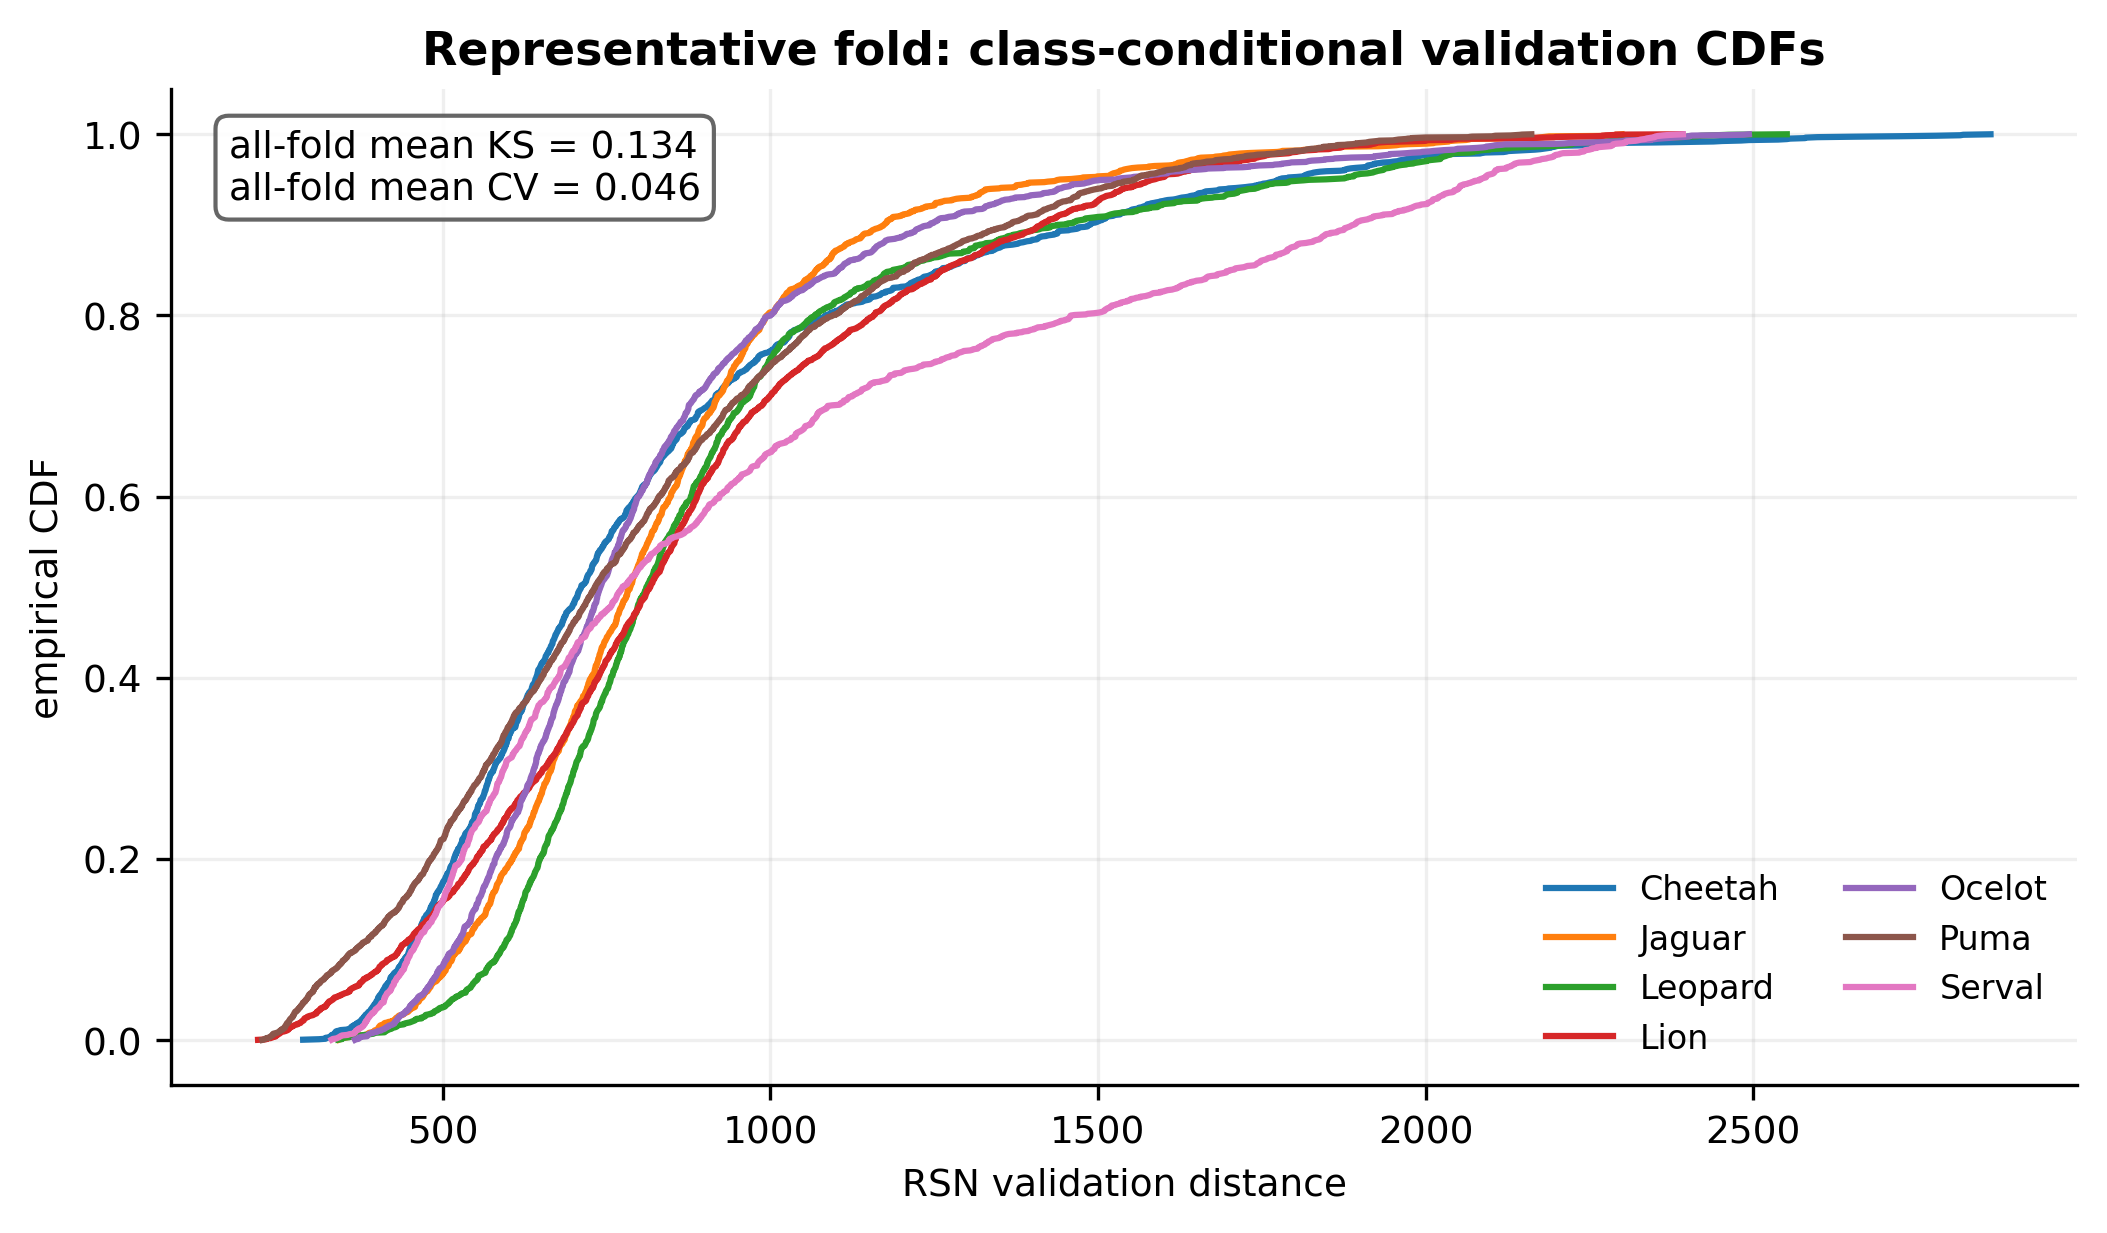
\includegraphics[width=\linewidth]{fig05_shared_shape_cdf.png}
  \caption{代表 fold のクラス別 validation 距離 CDF．数値は全1,476 foldの平均．}
  \label{fig:cdf}
\end{figure}

\subsection{Huber 化の役割}

Huber 化は全体平均では小さいが安定した改善を与える．未知種別には差があり，全 $m$ 集計で cheetah は AUROC $+0.0011$，tiger と lion は約 $+0.0006$，leopard は $-0.0003$ であった（付録図~\ref{fig:huber_species}）．これは，広い次元に分散した OOD 信号では単一座標ノイズの抑制が有効だが，少数次元へ集中した信号では線形化が検出力も抑えうるというトレードオフを示す．したがって Huber は主役の効果ではなく，対角標準化を安定化する小さな補助要素と位置づける．

\subsection{なぜ生特徴・全クラスが効くか}

DINOv2 特徴ノルムは画像品質，背景，対象の可視性などを含む可能性がある．$\ell_2$ 正規化は角度情報へ限定するため，超近接種を分ける補助信号も除去しうる．また top-3 候補制限は計算量を減らすが，未知入力に対する ridge head の誤順位を score へ持ち込む．本稿の主設定は両者を避ける．ただし表~\ref{tab:ablation}の別設定は3要因を同時に変えるため，どの要因が支配的かを確定するには raw/$\ell_2$，$k$，候補数を独立に振る追加実験が必要である．

\section{限界}

本研究には次の限界がある．第一に，単一のネコ科8種に限定しており，他科・他ドメインへの外的妥当性は未確認である．第二に，ウェブ収集画像を自動・目視規則でクリーニングしたが，細かな誤ラベルや低品質画像が残る可能性がある．第三に，完全な全手法ランキングは計算費用のため $m=2$ のみであり，$m=3$--7では \knn と PSM を主比較とした．第四に，ODIN と CLIP 系を無理に cached DINOv2 特徴へ移植せず除外したため，別 encoder を含む横断比較ではない．第五に，fold 間は同じ画像集合を異なる ID/OOD 組合せで再利用するため完全独立ではなく，paired CI は設定間依存を過小評価しうる．

\section{結論}

超近接 OOD に対し，クラス条件付き次元別標準化と Huber 集約を用いる \RSN を提示した．検証の結果，主設定は raw DINOv2 特徴，$k=150$，全 ID クラス，$\delta=1.345$，較正なしであり，過去に本文へ混入した $\ell_2$/10/top-3設定より明確に強かった．クリーニング後105,554枚の全1,476 foldで，\RSN は全 ID クラス数にわたり \knn と PSM を上回り，$m=2$ の検証済み全手法表でも最良だった．結果の再現性を担保するため，論文の数値は実装監査後の `verified\_v1' とクリーニング後集計だけへ限定した．

\appendix
\section{補足結果}

\begin{figure*}[t]
  \centering
  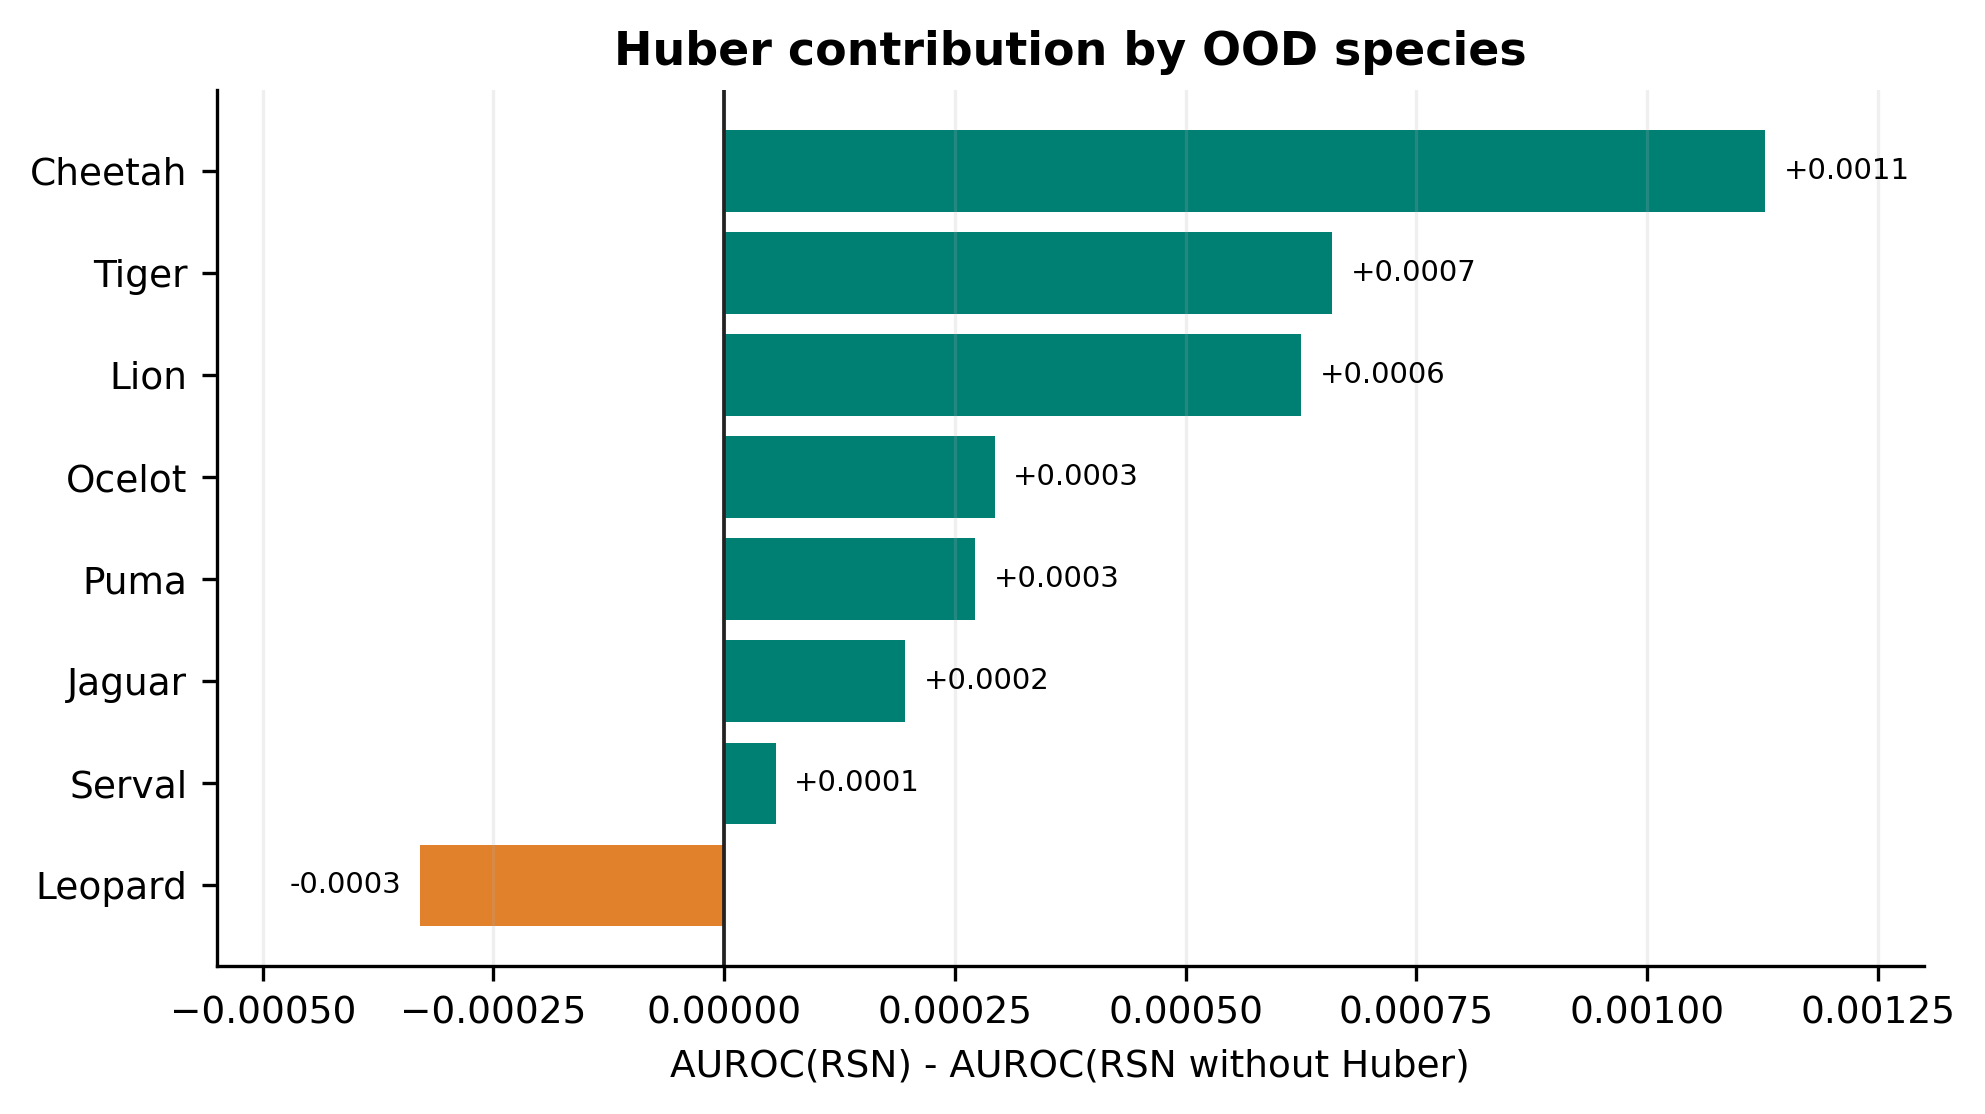
\includegraphics[width=0.78\textwidth]{fig06_huber_species.png}
  \caption{全 ID クラス数を併合した，Huber 化による未知種別 AUROC 差．}
  \label{fig:huber_species}
\end{figure*}

\begin{table*}[t]
\centering
\scriptsize
\caption{$m=2$ の検証済み全ランキング．RSN の $\ell_2$/10/top-3設定は手法ランキングから外し，表~\ref{tab:ablation}の設定感度としてのみ報告する．}
\label{tab:fullranking}
\begin{tabular}{clrrr@{\hspace{9mm}}clrrr}
\toprule
順位 & 手法 & AUROC & FPR95 & AUPR & 順位 & 手法 & AUROC & FPR95 & AUPR\\
\midrule
1 & \RSN & .9169 & .4307 & .9590 & 12 & Energy & .8439 & .5293 & .9356\\
2 & \knn & .9126 & .4626 & .9560 & 13 & GradNorm & .8430 & .5326 & .9350\\
3 & ViM & .9041 & .5436 & .9482 & 14 & SCALE & .8343 & .5425 & .9320\\
4 & Mahalanobis & .9010 & .5474 & .9470 & 15 & RMD & .8314 & .5694 & .9287\\
5 & Mahalanobis++ & .8987 & .5618 & .9453 & 16 & KL-Matching & .7996 & .5498 & .9201\\
6 & DICE & .8792 & .7230 & .9292 & 17 & NCI & .7989 & .6648 & .9043\\
7 & Entropy & .8440 & .5292 & .9357 & 18 & ReAct & .6006 & .8949 & .7888\\
8 & GEN & .8440 & .5292 & .9357 & 19 & ASH-B & .4957 & .9310 & .7524\\
9 & MSP & .8440 & .5292 & .9357 & 20 & ASH-P & .4934 & .9534 & .7381\\
10 & OpenMax & .8440 & .5293 & .9356 & 21 & ASH-S & .4879 & .9483 & .7395\\
11 & MaxLogit & .8440 & .5293 & .9356 & & & & &\\
\bottomrule
\end{tabular}
\end{table*}

\section{再現用設定}

主設定は \texttt{normalize=false, k=150, delta=1.345, min\_std=1e-3, candidate=all, calibrated=false} である．評価単位は \texttt{backbone, seed, id\_size, id\_set} の組であり，fold-level CSV は同じ単位で手法を paired に結合できる．検証済み実装は \texttt{src/maf07/methods/verified\_baselines.py}，監査 runner は \texttt{scripts/run\_verified\_baseline\_audit.py} に保存した．

\begin{thebibliography}{99}

\bibitem{hendrycks2017baseline}
D. Hendrycks and K. Gimpel,
``A Baseline for Detecting Misclassified and Out-of-Distribution Examples in Neural Networks,''
\textit{ICLR}, 2017.

\bibitem{norouzzadeh2018automatically}
M. S. Norouzzadeh et al.,
``Automatically identifying, counting, and describing wild animals in camera-trap images with deep learning,''
\textit{PNAS}, vol. 115, no. 25, 2018.

\bibitem{tuia2022perspectives}
D. Tuia et al.,
``Perspectives in machine learning for wildlife conservation,''
\textit{Nature Communications}, vol. 13, 2022.

\bibitem{sun2022knn}
Y. Sun, Y. Ming, X. Zhu, and Y. Li,
``Out-of-Distribution Detection with Deep Nearest Neighbors,''
\textit{ICML}, 2022.

\bibitem{liu2020energy}
W. Liu, X. Wang, J. Owens, and Y. Li,
``Energy-based Out-of-distribution Detection,''
\textit{NeurIPS}, 2020.

\bibitem{liu2023gen}
X. Liu, Y. Lochman, and C. Zach,
``GEN: Pushing the Limits of Softmax-Based Out-of-Distribution Detection,''
\textit{CVPR}, 2023.

\bibitem{huang2021gradnorm}
R. Huang, A. Geng, and Y. Li,
``On the Importance of Gradients for Detecting Distributional Shifts in the Wild,''
\textit{NeurIPS}, 2021.

\bibitem{bendale2016openmax}
A. Bendale and T. Boult,
``Towards Open Set Deep Networks,''
\textit{CVPR}, 2016.

\bibitem{lee2018simple}
K. Lee, K. Lee, H. Lee, and J. Shin,
``A Simple Unified Framework for Detecting Out-of-Distribution Samples and Adversarial Attacks,''
\textit{NeurIPS}, 2018.

\bibitem{ren2021simple}
J. Ren et al.,
``A Simple Fix to Mahalanobis Distance for Improving Near-OOD Detection,''
\textit{ICML Workshop}, 2021.

\bibitem{muller2025mahalanobispp}
M. M\"uller and M. Hein,
``Mahalanobis++: Improving OOD Detection via Feature Normalization,''
\textit{ICML}, 2025.

\bibitem{wang2022vim}
H. Wang, Z. Li, L. Feng, and W. Zhang,
``ViM: Out-of-Distribution with Virtual-Logit Matching,''
\textit{CVPR}, 2022.

\bibitem{oquab2024dinov2}
M. Oquab et al.,
``DINOv2: Learning Robust Visual Features without Supervision,''
\textit{TMLR}, 2024.

\bibitem{huber1964robust}
P. J. Huber,
``Robust Estimation of a Location Parameter,''
\textit{The Annals of Mathematical Statistics}, vol. 35, no. 1, 1964.

\bibitem{dkw1956}
A. Dvoretzky, J. Kiefer, and J. Wolfowitz,
``Asymptotic Minimax Character of the Sample Distribution Function and of the Classical Multinomial Estimator,''
\textit{The Annals of Mathematical Statistics}, vol. 27, no. 3, 1956.

\end{thebibliography}

\end{document}
